\documentclass[10pt,letterpaper,final,twoside,notitlepage]{article}
\usepackage[margin=.5in]{geometry}
\usepackage[utf8]{inputenc}
\usepackage[english]{babel}
\usepackage{amsmath}
\usepackage{amsfonts}
\usepackage{amssymb}
\usepackage{graphicx}

\usepackage{subcaption} % Float environment to place multiple figures in one figure environment
\usepackage{nameref} % \nameref{label} lets you reference things by name
\usepackage{hyperref} % Hyperlinks between references
\usepackage{textcomp} % Forcibly loads a dependency for gensymb
\usepackage{gensymb} % Gives us access to some other symbols
\usepackage{siunitx} % Gives access to SI units
\usepackage{enumitem} % Provides [noitemsep, nolistsep] for more compact lists
\usepackage{multicol} % Allows me to split portion of a page into multiple columns

\graphicspath{{./Drawings/ECE_213/}} % Uncomment this to use pictures in this document
%\numberwithin{equation}{section} % Uncomment this to number equations with section numbers too

\renewcommand{\Re}{\operatorname{Re}} % Redefine to use the command, but not the fraktur version
\renewcommand{\Im}{\operatorname{Im}} % Redefine to use the command, but not the fraktur version
\DeclareMathOperator{\Lapl}{\mathcal{L}} % Declare a Laplace symbol to be used
\DeclareMathOperator{\UnitStep}{\mathcal{U}} % Delare a unit step function symbol

\author{Karl Hallsby}
\title{ECE 213 Equations}

\begin{document}
	
%\section*{General Equations}
	\begin{itemize}[noitemsep] % Basic Equations
		\item KCL: $\sum I_{in} = \sum I_{Out}$ $\rightarrow$ Node's Input Current = Node's Output Current
		\item KVL: $\sum V = 0$ $\rightarrow$ Voltage across a loop totals to 0.
		\item Ohm's Law: $V=IR$
	\end{itemize}
	\vspace{-5mm}

\section*{Phasors} \label{sec:Phasors}
Phasors will only show us the steady state response of the circuit, not the transient response. \newline 
\textbf{\large Eq: $v(t)=V_{M} \cos \left(\omega t + \theta \right)$ $\leftrightarrow$ $\bar{V}=V_{M} \angle \theta_{v} = V_{M}e^{\jmath \theta_{v}} = V_{M}\left(\cos \theta_{v} + \jmath \sin \theta_{v}\right)$} \newline
You can use phasors with \nameref{subsec:Nodal Analysis}, \nameref{subsec:Mesh Analysis}, \nameref{subsec:Superposition}, and \nameref{sec:Thevenin/Norton}. \newline
	\begin{table}[ht] % Phasor Operation Table
		\centering
		\renewcommand{\arraystretch}{1.4}
		$z_1=x_1+\jmath y_2=r_1\angle\phi_1$, $z_2=x_2+\jmath y_2=r_2\angle\phi_2$
		\begin{tabular}{|c|c|} 
			\hline
			Addition & $z_1+z_2=\left( x_1+x_2 \right)+ \jmath \left( y_1+y_2 \right)$ \\ \hline
			Subtraction & $z_1-z_2=\left( x_1-x_2 \right)+ \jmath \left( y_1-y_2 \right)$ \\ \hline
			Multiplication & $z_{1}z_{2}=r_{1}r_{2}\angle \left( \phi_1 + \phi_2 \right)$ \\ \hline
			Division & $\frac{z_{1}}{z_{2}} = \frac{r_{1}}{r_{2}} \angle \left(\phi_1 - \phi_2 \right)$ \\ \hline
			Reciprocal & $\frac{1}{z_1}=\frac{1}{z_1} \angle -\phi_1$ \\ \hline
			Square Root & $\sqrt{z_1}=\sqrt{r_1} \angle \frac{\phi_1}{2}$ \\ \hline
			Complex Conjugate & $ z_1^*=x- \jmath y=r \angle -\phi_1=re^{-\jmath \phi_1}$\\ \hline
		\end{tabular}
	\end{table}
	\vspace{-8mm}

\section*{RMS/Complex Power/Max Power Transfer} \label{sec:Complex Power}
	\vspace{-6mm}
	\begin{multicols}{2}
		\begin{itemize}[noitemsep]
			\item $X_{rms}=\sqrt{\frac{1}{T} \int_{0}^{T} x(t)^2 dt}=\frac{X_{PP}}{2 \sqrt{2}}=\frac{X_{PP}}{2 \sqrt{2}}$
			\item $P_{avg}=\frac{1}{2} \Re\lbrace \mathbf{V} \mathbf{I}^* \rbrace=\frac{1}{2}V_{m}I_{m}\cos \left(\theta_v -\theta_i \right)$
			\item $\mathbf{S} = I_{rms}^2\mathbf{Z} = \frac{V_{rms}^2}{\mathbf{Z}^*} = \mathbf{V}_{rms}\mathbf{I}_{rms}^*$ \vspace{1.2mm}
			\item $\sum_{k=1}^{n} S_{k}$ \vspace{1.2mm}
			\item $C = \frac{Q_{C}}{\omega V_{rms}^2} = \frac{P\left( \tan \theta_1 - \tan \theta_2 \right)}{\omega V_{rms}^2}$ \vspace{1.2mm}
			\item $L=\frac{V_{rms}^2}{\omega \left(Q_1 - Q_2 \right)}$
		\end{itemize}

		\columnbreak
		
		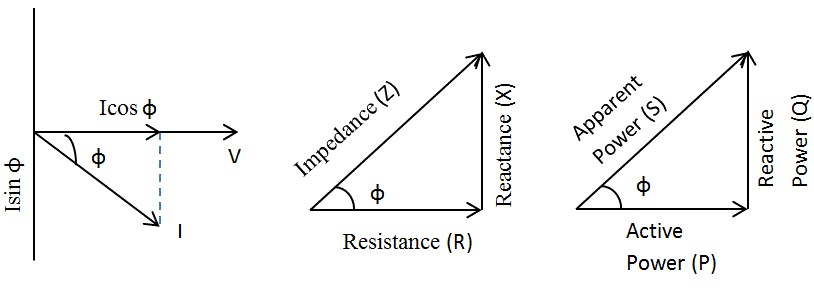
\includegraphics[scale=0.375]{Phasor_Power_Triangle.jpg} % Can't do figure because floats aren't allowed in multicol
		\label{fig:Phasor/Power Triangle}
	\end{multicols}
	\vspace{-4mm}

	\begin{table}[h!] % Complex Power Table
		\centering
		\renewcommand{\arraystretch}{1.4}
		\begin{tabular}{|c|c|c|c|}
			\hline
			\textbf{Name} & \textbf{Symbol} & \textbf{Equation(s)} & \textbf{Units} \\ \hline
			Complex Power & $\mathbf{S}$ & $\frac{P}{Pf} \angle\arccos\left( Pf\right)=P+\jmath Q=\mathbf{V}_{rms} \mathbf{I}_{rms}^{*} = \lvert \mathbf{V}_{rms}\rvert \lvert \mathbf{I}_{rms}\rvert \angle \left( \theta_v - \theta_i\right) $ & \si{\volt \ampere} \\ \hline
			Apparent Power & $S$ & $\lVert \mathbf{S} \rVert = \lvert \mathbf{V}_{rms} \rvert \lvert \mathbf{I}_{rms} \rvert = \sqrt{P^2 + Q^2}$ & \si{\volt \ampere} \\ \hline
			Real Power & $P$ & $\Re\lbrace \mathbf{S} \rbrace = S * Pf \cos \left[ \arccos \left( Pf \right) \right] = S \cos\left( \theta_v - \theta_i \right)$ & \si{\watt} \\ \hline
			Reactive (Imaginary) Power & $Q$ & $\Im\lbrace \mathbf{S} \rbrace = S * Pf \sin \left[ \arccos \left( Pf \right) \right] =  S \sin \left( \theta_v - \theta_i \right)$ & \si{VAR}\\ \hline
			Power Factor &\textit{Pf} & $\frac{P}{S} = \cos(\theta_v - \theta_i)$ & Lead/Lag \\ \hline
		\end{tabular}
	\end{table}
	\textbf{NOTE:} If you are looking for 3-Phase complex power, it is in \nameref{sec:3-Phase}.
	\vspace{-4mm}

\section*{Elements} \label{sec:Circuit Elements}
	\begin{table}[h!] % Element Equation Table
		\centering
		\renewcommand{\arraystretch}{1.4}
		\begin{tabular}{|c|c|c|c|}
		\hline
		Relation & R & C & L \\
		\hline
		v-i & $V=IR$ & $v = \frac{1}{C} \int_{t_0}^t i(x)dx + v(t_0)$ & $v=L\frac{di}{dt}$  \\
		i-v & $I=\frac{V}{R}$ & $i = C\frac{dv}{dt}$ & $i=\frac{1}{L}\int_{t_0}^t v(x)dx +i(t_0)$ \\
		\hline
		P or W & $P=I^2R=\frac{V^2}{R}$ & $P=\frac{1}{2}Cv_{c}^2$ & $W=\frac{1}{2}Li_{l}^2$ \\
		\hline
		Series & $R_{eq}=R_1+R_2+\ldots+R_n$ & $\frac{1}{C_{eq}}=\frac{1}{C_1}+\frac{1}{C_2}+\ldots+\frac{1}{C_n}$ & $L_{eq}=L_1+L_2+\ldots+L_n$ \\
		Parallel & $\frac{1}{R_{eq}}=\frac{1}{R_1}+\frac{1}{R_2}+\ldots+\frac{1}{R_n}$ & $C_{eq}=C_1+C_2+\ldots+C_n$ & $\frac{1}{L_{eq}}=\frac{1}{L_1}+\frac{1}{L_2}+\ldots+\frac{1}{L_n}$ \\
		\hline
		@ Steady State & Same (Nothing Happens) & Open Circuit & Short Circuit \\
		\hline
		Phasors & $Z_R=R$ & $Z_C = \frac{1}{j \omega C}$ & $Z_L=j \omega L$ \\
		\hline
		\end{tabular}
	\end{table}

%\section*{Methods to Solve Equations} \label{sec:Solve Circuits}
	\subsection*{Nodal Analysis} \label{subsec:Nodal Analysis}
		\begin{enumerate}[noitemsep, nolistsep]
			\item \# of Nodes? $\rightarrow n$
			\item Make one node the reference node. Assign $n-1$ nodal voltages
			\item For a \textbf{voltage} source, write a CONSTRAINT EQUATION (Con. Eq.). If there is a voltage source between 2 non-reference nodes, make that a \textbf{SUPERNODE}.
			\item Write KCL at each node. ($n-1$) equations.
			\item Solve Equations.
		\end{enumerate}
	\subsection*{Mesh/Loop Analysis} \label{subsec:Mesh Analysis}
		\begin{enumerate}[noitemsep, nolistsep]
			\item \# of Nodes? $\rightarrow n$ \# of Branches? $\rightarrow b$ \# of meshes/loops? $\rightarrow b-n+1 = l$
			\item Assign $l$ loop currents.
			\item For \textbf{current} sources, write a CONSTRAINT EQUATION (Con. Eq.). If there is a current source between 2 meshes, that's a \textbf{SUPERMESH}.
			\item Write KVL for each mesh.
			\item Solve Equations.
		\end{enumerate}
	\subsection*{Superposition} \label{subsec:Superposition}
		\begin{itemize}[noitemsep, nolistsep]
			\item \# of sources, $n$, determines the number of equations you will have.
			\item Shut off each source, one at a time, solving for the term that you want.
			\begin{itemize}[noitemsep, nolistsep]
				\item Voltage Source = S.C.
				\item Current Source = O.C.
			\end{itemize}
			\item Sum each of the individual terms together. $\sum_{i=1}^{n} x_{i}$ \vspace{1.5mm}
			\item \textbf{\large THIS IS THE ONLY WAY TO SOLVE FOR A CIRCUIT WITH MULTIPLE SOURCES!!}
		\end{itemize}

	\subsection*{Source Transformations} \label{sec:Source Transforms}
		\textbf{ALL} source transformations obey Ohm's Law. $V=IR$.
		This will \textbf{ONLY} work on impedances in series with \textbf{VOLTAGE} sources, or impedances in parallel with \textbf{CURRENT} sources.
		\vspace{-5mm}

\section*{Thevenin and Norton Equivalencies} \label{sec:Thevenin/Norton}
	\begin{itemize}[noitemsep, nolistsep]
		\item ONLY independent sources - Zero all sources, find $\mathbf{Z}_{eq}$.
		\begin{itemize}[noitemsep, nolistsep] % Zero Sources
			\item 0-ing Current Sources = O.C., 0-ing Voltage Sources = S.C.
			\item Look at circuit from load's perspective for $\mathbf{Z}_{eq}$
			\item $\mathbf{V}_{Th}=\mathbf{V}_{OC}$, $\mathbf{I}_{N} = \mathbf{I}_{SC}$
		\end{itemize}
		\item BOTH dependent and independent sources
			\begin{itemize}[noitemsep, nolistsep] % Voc/Isc
				\item Find $\mathbf{V}_{Th}=\mathbf{V}_{OC}$, $\mathbf{I}_{N}=\mathbf{I}_{SC}$
				\item Solve $\mathbf{Z}_{Th}=\frac{\mathbf{V}_{OC}}{\mathbf{I}_{SC}}$
			\end{itemize}
		\item ONLY dependent sources
			\begin{itemize}[noitemsep, nolistsep] % Test Source
				\item $\mathbf{V}_{Th}=0$, $\mathbf{I}_{N}=0$
				\item $\mathbf{Z}_{Th}=\mathbf{Z}_{N} \rightarrow$ Attach test source @ load.
				\begin{itemize}
					\item If voltage test source, find current. If current test source, find voltage
				\end{itemize}
				\item $\mathbf{Z}_{Th}=\frac{\mathbf{V}_{Test}}{\mathbf{I}_{Test}}$
			\end{itemize}
		\end{itemize}
	\vspace{-5mm}
	
\section*{Maximum Power Transfer - AC}
	\begin{itemize}[noitemsep, nolistsep]
		\item $\mathbf{Z}_{Load}=\mathbf{Z}_{Th}^*$, $R_{Th}=\Re\lbrace\mathbf{Z_{Th}}\rbrace$, $R_L= \lvert \mathbf{Z}_{Th} \rvert = \sqrt{R_{Th}^2+\left( X_{Th}+X_{L}\right)^2}$
		\item $P_{max}=\frac{\lvert\mathbf{V}_{Th}\rvert^2}{8R_{Th}}$
	\end{itemize}
	\vspace{-4.5mm}
\section*{3-Phase Circuits} \label{sec:3-Phase}
	\begin{figure} % 3 Phase Configurations
		\begin{subfigure}{0.5\textwidth} % 3 Phase Y
			\centering
			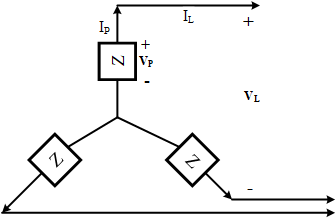
\includegraphics[scale=0.4]{3Phase-Y.png}
			\subcaption{\textbf{3 Phase $Y$-Connection}}
			\label{subfig:3 Phase-Y}
			\begin{align*}
				I_{L} &= I_{P} &
				V_{LL} &= \sqrt{3} V_{P} \angle \ang{30} &
				Z_{Y} &= \frac{Z_{\Delta}}{3} \\
				\mathbf{S} &= \sqrt{3} \mathbf{V}_{L} \mathbf{I}_{L}^{*} &
				\mathbf{S} &= 3 \mathbf{V}_{P} \mathbf{I}_{L}^{*} &
				\phi &= \theta_{V_{P}} - \theta_{I_{P}} \\
				\mathbf{S} &= S \angle \phi &
				P &= \lVert \mathbf{S} \rVert \cos \left( \phi \right) &
				Q &= \lVert \mathbf{S} \rVert \sin \left( \phi \right) \\
			\end{align*}
		\end{subfigure}
		\vline
		\begin{subfigure}{0.5\textwidth} % 3 Phase Delta
			\centering
			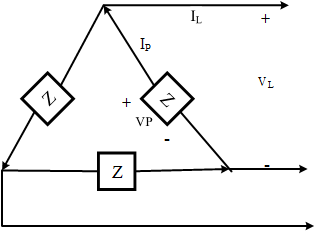
\includegraphics[scale=0.4]{3Phase-Delta.png}
			\subcaption{\textbf{3 Phase $\Delta$-Connection}}
				\begin{align*}
					I_{L} &= \sqrt{3} I_{P} \angle \ang{-30} &
					V_{LL} &= V_{P} &
					Z_{\Delta} &= 3 Z_{Y} \\
					\mathbf{S} &= \sqrt{3} \mathbf{V}_{L} \mathbf{I}_{L}^{*} &
					\mathbf{S} &= 3 \mathbf{V}_{P} \mathbf{I}_{P}^{*} &
					\phi &= \theta_{V_{P}} - \theta_{I_{P}} \\
					\mathbf{S} &= S \angle \phi &
					P &= \lVert \mathbf{S} \rVert \cos \left( \phi \right) &
					Q &= \lVert \mathbf{S} \rVert \sin \left( \phi \right) \\
				\end{align*}
			\label{subfig:3 Phase-Delta}
		\end{subfigure}
	\end{figure}
\begin{itemize}[noitemsep, nolistsep]
	\item $C_{Y} = \frac{Q_{C}}{3 \omega \lVert V_{\phi,rms} \rVert^{2}}$
	\item $C_{\Delta} = \frac{C_{Y}}{3}$
	\item Power lost due to line: $P_{Lost}=Z_{Wire}I_{L}$
\end{itemize}
You want to get everything into Y formation, because the common neutral allows you to do single-phase analysis.
\vspace{-5mm}

\section*{Mutual Inductance} \label{sec:Mutual Inductance}
	\subsection*{Equivalent Mutual Inductance}
		\begin{table}[h!] % Mutual Inductance Equivalency Table
			\centering
			\renewcommand{\arraystretch}{2.25}
			\begin{tabular}{|c|c|c|}
			\hline
			Series-\textbf{Aiding} Connection & $L=L_{1}+L_{2}+2M$ & 
\includegraphics[scale=0.35]{Mutual_Inductors_Series_Dots_Aiding.png} \\ \hline
			Series-\textbf{Opposing} Connection & $L=L_{1}+L_{2}-2M$ & 
\includegraphics[scale=0.35]{Mutual_Inductors_Series_Dots_Opposing.png} \\ \hline
			\end{tabular}
		\end{table}

	\subsection*{Dot Convention} \label{subsec:Dot Convention}
		There are 2 cases:
		\begin{enumerate}[noitemsep, nolistsep]
			\item Current enters through dotted side on 1 inductor $\longrightarrow$ \textbf{POSITIVE VOLTAGE ON DOTTED SIDE OF OTHER INDUCTOR}
				\begin{itemize}[noitemsep, nolistsep]
					\item Current flows into the dotted side of one inductor
					\item Current flows out of the un-dotted side of second inductor, just like the first
				\end{itemize}
			\item Current enters through \textbf{NON}-dotted side of 1 inductor $\longrightarrow$ \textbf{POSITIVE VOLTAGE ON UN-DOTTED SIDE OF OTHER INDUCTOR}
				\begin{itemize}[noitemsep, nolistsep]
					\item Current flows into the un-dotted side of one inductor
					\item Current flows out of the dotted side of the second inductor, just like the first
				\end{itemize}
		\end{enumerate}
	
	\subsection*{Solving Disjoint Coupled Circuits} \label{subsec:Solve Disjoint Coupled Circuits}
		\begin{enumerate}[noitemsep] % Steps
			\item Apply KVL
			\item Don't forget about the Mutual Inductance Voltage Difference because of the first current
			\item There is a second way to thing about these, shown in Figures~\ref{subfig:Disjoint Coupled Inductors OG}~and~\ref{subfig:Disjoint Coupled Inductors Simplified}, below.
		\end{enumerate}
		\begin{figure}[ht!] % Convert
			\begin{subfigure}{0.5\textwidth}
				\centering
				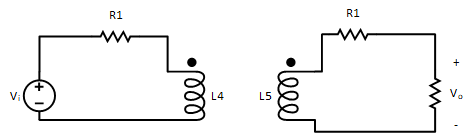
\includegraphics[scale=0.35]{Disjoint_Coupled_Inductors-OG.png}
				\subcaption{Original Circuit}
				\label{subfig:Disjoint Coupled Inductors OG}
			\end{subfigure}
			\begin{subfigure}{0.5\textwidth}
				\centering
				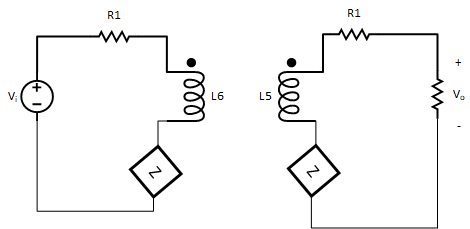
\includegraphics[scale=0.30]{Disjoint_Coupled_Inductors-Simplified.png}
				\subcaption{Circuit "Simplified" by Adding Dependent Sources}
				\label{subfig:Disjoint Coupled Inductors Simplified}
			\end{subfigure}
		\end{figure}
		\textbf{The sign on the dependent sources depends on which side of the inductor the current is going into.} \newline
		\textbf{Use the \nameref{subsec:Dot Convention} to determine which direction the source's voltage should go.}
	\vspace{-6mm}

\section*{Transformers} \label{sec:Transformers}
These elements consume no power, and convert voltages and currents.
\begin{itemize}[noitemsep, nolistsep]
	\item $\frac{v_{1}}{v_{2}} = \frac{N_{1}}{N_{2}} \longleftarrow$ Voltage Change
	\item $\frac{i_{1}}{i_{2}} = -\frac{N_{2}}{N_{1}} \longleftarrow$ Current Change
\end{itemize}
\vspace{-4.75mm}

	\subsection*{Representations for Turns} \label{subsec:Turn Representations}
		There are 3 common ways to represent the number of turns in a transformer:
		\begin{enumerate}[noitemsep, nolistsep]
			\item $N_{1} : N_{2}$
			\begin{itemize}[noitemsep, nolistsep]
				\item Both $N_{1}$ and $N_{2}$ are integers
			\end{itemize}
			\item $1 : n$
			\begin{itemize}[noitemsep, nolistsep]
				\item The first term might not be $1$, if there isn't perfect division, i.e. $2 : 5$ will not be reduced to $1 : \frac{5}{2}$
				\item $n = \frac{N_{2}}{N_{1}}$
				\item This is the form generally used by our textbook
			\end{itemize}
			\item $a : 1$
			\begin{itemize}[noitemsep, nolistsep]
				\item The second term might not be $1$, if there isn't perfect division, i.e. $2 : 5$ will not be reduced to $\frac{2}{5} : 1$
				\item $a = \frac{N_{1}}{N_{2}}$
				\item This is the form generally used by utility companies
			\end{itemize}
		\end{enumerate}
		\vspace{-5mm}
		
	\subsection*{Reflecting Elements} \label{subsec:Element Reflection}
		There are only 3 equations:
		\begin{enumerate}[noitemsep, nolistsep]
			\item $\frac{v_{1}}{v_{2}} = \frac{N_{1}}{N_{2}} \longleftarrow$ Voltage Change
			\item $\frac{i_{1}}{i_{2}} = -\frac{N_{2}}{N_{1}} \longleftarrow$ Current Change
			\item $Z_{1} = \frac{Z_{2}}{n^{2}}$, as seen in Figure~\ref{fig:Transformer Reflecting}
			\item A negative can be in any one of these, depending on the dot orientation
		\end{enumerate}
		\begin{figure}[ht!]
			\centering
			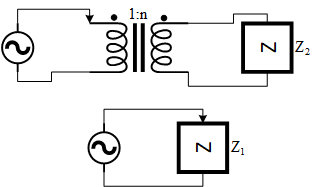
\includegraphics[scale=0.375]{Transformer_Reflecting.png}
			\caption{Transformer Reflecting Elements}
			\label{fig:Transformer Reflecting}
		\end{figure}
		\vspace{-10mm}
	
\section*{Transfer Functions/Bode Plots} \label{sec:Bode Plots}
	\begin{itemize}[noitemsep, nolistsep]
		\item Basic form of a Transfer function is $H \left( \omega \right) = \frac{X_{Out}}{X_{In}}$
		\begin{itemize}[noitemsep, nolistsep]
			\item $H \left( \omega \right) = \frac{V_{Out}}{V_{In}}$
			\item $H \left( \omega \right) = \frac{I_{Out}}{I_{In}}$
			\item $H \left( \omega \right) = \frac{V_{Out}}{I_{In}}$
			\item $H \left( \omega \right) = \frac{I_{Out}}{V_{In}}$
		\end{itemize}
	\end{itemize}
	We replace {\large $s = \omega j \rightarrow \omega = \frac{s}{j}$}. \newline
	When we have the transfer function, and plug in the equivalency $s = \omega j$, we end up with something like:
	\begin{equation*}
		H\left( s \right) = \frac{k \left(s + z_{1} \right) \left(s + z_{2} \right) \left(s + z_{3} \right) \cdots}{\left(s + p_{1} \right) \left(s + p_{2} \right) \left(s + p_{3} \right) \cdots}
	\end{equation*}
	Now to make the bode plot:
	\begin{align*} % Construct Bode Equations
		\lVert H\left( s \right) \rVert &= \frac{k \lVert s + z_{1} \rVert \lVert s + z_{2} \rVert \lVert s + z_{3} \rVert \cdots}{\lVert s + p_{1} \rVert \lVert s + p_{2} \rVert \lVert s + p_{3} \rVert \cdots} \\
		\lVert H\left( \omega \right) \rVert (dB) &= 20\log \left( k \right) + 20\log \left( j\omega + z_{1} \right) + 20\log \left( j\omega + z_{2} \right) + 20\log \left( j\omega + z_{3} \right) \\
		&- 20\log \left( j\omega + p_{1} \right) - 20\log \left( j\omega + p_{2} \right) - 20\log \left( j\omega + p_{3} \right) \\
		\angle \varphi &= \arctan \left( k \right) + \arctan \left( j\omega + z_{1} \right) + \arctan \left( j\omega + z_{2} \right) + \arctan \left( j\omega + z_{3} \right) \\
		&-\arctan \left( j\omega + p_{1} \right) - \arctan \left( j\omega + p_{2} \right) - \arctan \left( j\omega + p_{3} \right) \\
	\end{align*}
	\vspace{-12mm}
	\begin{table}[!h]% Bode Plot Table
		\centering
		\renewcommand{\arraystretch}{2.35}
		\begin{tabular}{|c|c|c|} % Bode Plot Table
			\hline
			\textbf{Factor} & \textbf{Magnitude} $\lVert H\left( \omega \right) \rVert (dB)$ & \textbf{Phase} $ \angle \varphi$ \\ \hline
			%---------------------------------------------------------------------------%
			$K$ & $20 \log_{10} K$ & $0 \degree$ \\ \hline
			$\left( j \omega \right)^{N}$ & $ 20N \text{dB/decade}$ (Passes through 1 and continues) & $90N \degree$ \\ \hline
			$\frac{1}{\left( j \omega \right)^{N}}$ & $-20N \text{dB/decade}$ (Passes through 1 and continues) & $-90N \degree$ \\ \hline
			
			$\left( 1 + \frac{j \omega}{z} \right)^{N}$ &
				$\begin{cases}
					0 & x \leq z \\
					20N \text{dB/decade} \\
				\end{cases}$ 
				&
				$\begin{cases}
					0 & < \frac{z}{10} \\
					\frac{1}{2} \left( 90N \right) \degree & =z \\
					90N \degree & \geq 10z \\
				\end{cases}$ 
				\\ \hline
				
				$\frac{1}{\left( 1 + j \omega / p \right)^{N}}$ & 
					$\begin{cases}
							0 & x \leq z \\
							-20N \text{dB/decade} \\
						\end{cases}$ 
					& 
					$\begin{cases}
						0 & < \frac{z}{10} \\
						\frac{1}{2} \left( -90N \right) \degree & =z \\
						-90N \degree & \geq 10z \\
					\end{cases}$ 
					\\ \hline
				
				$\left[ 1 + \frac{2 j \omega \zeta}{\omega_{n}} + \left( \frac{j \omega}{\omega_{n}} \right)^{2} \right]^{N}$ & $\begin{cases}
					0 & \leq \omega_{n} \\
					40N \text{dB/decade} & > \omega_{n} \\
				\end{cases}$
				&
				$\begin{cases}
					0 & \leq \frac{\omega_{n}}{10} \\
					\frac{1}{2} \left( 180 N \right) \degree & = \omega_{n} \\
					180N \degree & \geq 10 \omega_{n} \\
				\end{cases}$
				\\ \hline
				
				$\frac{1}{\left[ 1 + \frac{2 j \omega \zeta}{\omega_{k}} + \left( j \omega / \omega_{k} \right)^{2} \right]^{N}}$ & $\begin{cases}
					0 & \leq \omega_{k} \\
					-40N \text{dB/decade} & > \omega_{k} \\
				\end{cases}$
				&
				$\begin{cases}
					0 & \leq \frac{\omega_{n}}{10} \\
					\frac{1}{2} \left( -180 N \right) \degree & = \omega_{k} \\
					-180N \degree & \geq 10 \omega_{k} \\	
				\end{cases}$
				\\ \hline
		\end{tabular}
	\end{table}
\vspace{-5mm}

%\clearpage
\section*{Resonant Frequencies} \label{sec:Frequency Resonance}
Remember, $\omega = 2 \pi f$.
Also, $\Im \lbrace Z_{eq} \rbrace = 0$ and $\Im \lbrace Y_{eq} \rbrace = 0$.
\begin{itemize}[nolistsep]
	\item $\omega_{0} = \frac{1}{\sqrt{LC}}$ - Imaginary portion of Transfer function vanishes
	\item Half-Power Frequencies - Frequencies where power dissipated is 1/2 of that dissipated at resonant frequency
	\begin{itemize}[noitemsep]
		\item $\omega_{1} = - \frac{R}{2L} + \sqrt{\left( \frac{R}{2L} \right)^{2} + \frac{1}{LC}}$
		\item $\omega_{2} = \frac{R}{2L} + \sqrt{\left( \frac{R}{2L} \right)^{2} + \frac{1}{LC}}$
		\item $\omega_{0} = \sqrt{\omega_{1}\omega_{2}}$
	\end{itemize}
	\item $B = \omega_{2} - \omega_{1} = \frac{R}{L}$ - Bandwidth is the frequency band between half-power frequencies
	\begin{itemize}[noitemsep]
		\item $B = \frac{R}{L}$ - Series Impedance Circuit
		\item $B = \frac{1}{RC}$ - Parallel Impedance Circuit
	\end{itemize}
	\item $Q = \frac{\omega_{0}}{B}$ - Quality Factor: Sharpness of resonance peak
	\begin{itemize}[noitemsep]
		\item $Q =\frac{\omega_{0}L}{R} = \frac{1}{\omega_{0}RC}$ - Series Impedance Circuit
		\item $Q = \omega_{0}RC = \frac{R}{\omega_{0}L}$ - Parallel Impedance Circuit
	\end{itemize}
\end{itemize}
\vspace{-5mm}
\clearpage
\section*{Laplace Transform} \label{sec:Laplace Transform}
	\vspace{-2mm}
	\subsection*{Laplace Transform Properties} \label{subsec:Laplace Transform Properties}
		\vspace{-2mm}
		\begin{table}[h!]
			\renewcommand{\arraystretch}{1.4}
			\begin{tabular}{|l|c|c|}
				\hline
				\multicolumn{1}{|c|}{\textbf{Property Name}} & \multicolumn{1}{|c|}{\textbf{Time Domain}}& \multicolumn{1}{|c|}{\textbf{Frequency Domain}} \\ \hline
				Laplace Transform & $x(t) = \frac{1}{2j\pi} \int_{\sigma-\infty}^{\sigma+\infty} X(s) e^{st} ds$ & $X(s) = \int_{0^{-}}^{\infty} x(t) e^{-st} dt$ \\ \hline
				Linearity & $x(t) = \alpha_{1} x_{1}(t) + \alpha_{2} x_{2}(t)$ & $X(s) = \alpha X_{1}(s) + \alpha_{2} X_{2}(s)$ \\ \hline
				Time Scaling & $x(at) \text{, where } a>0$ & $\frac{1}{a} X \left( \frac{s}{a} \right)$ \\ \hline
				Time Shift & $x(t-a) \text{, where } a>0$ & $X(s)e^{-as}$ \\ \hline
				Frequency Shift & $x(t)e^{at}$ & $X(s)(s-a)$ \\ \hline
				Multiplication by $\sin \left( \omega_{0} t \right)$ & $x(t) \sin \left( \omega_{0} t \right)$ & $\frac{j}{2} \left[  X(s+j\omega_{0}) - X(s-j\omega_{0}) \right]$ \\ \hline
				Multiplication by $\cos \left( \omega_{0} t \right)$ & $x(t) \cos \left( \omega_{0} t \right)$ & $\frac{j}{2} \left[  X(s+j\omega_{0}) + X(s-j\omega_{0}) \right]$ \\ \hline
				Multiply by t in Time, Derivative in Frequency & $t^{n} x(t)$ & $(-1)^{n} \frac{d^{n}}{ds^{n}} X(s)$ \\ \hline
				Mutliply by s in Frequency, Derivative in Time & $\frac{d^{n}}{dt^{n}} x(t)$ & $s^{n}X(s) - \sum_{i=0}^{n-1} s^{n-1-i} \frac{d^{i}}{dt^{i}} x(t) \vert_{t=0^{-}}$ \\ \hline
				Integration & $\int_{0}^{t} x \left( \lambda \right) d\lambda$ & $\frac{1}{s} X(s)$ \\ \hline
				Multiply in Frequency, Convolution in Time & $x(t) * v(t)$ & $X(s)V(s)$ \\ \hline
				Initial Value Theorem & \multicolumn{2}{c|}{$x \left( 0^{+} \right) = \lim\limits_{s \rightarrow \infty} sX(s)$} \\ \hline
				Final Value Theorem & \multicolumn{2}{c|}{$\lim\limits_{t \rightarrow \infty} x(t) = \lim\limits_{s\rightarrow 0} sX(s)$} \\ \hline
				Relation to Fourier Transform & \multicolumn{2}{c|}{If $X(\omega)$ exists, then $X(s) = X(\omega)|_{\omega = \frac{s}{j}}$} \\ \hline
			\end{tabular}
		\end{table}
		\vspace{-5mm}
		
	\subsection*{Laplace Transform Pairs} \label{subsec:Laplace Transform Pairs}
		\begin{align*}
			\Lapl \lbrace x (t) \rbrace &= X(s) & \Lapl \lbrace \delta (t) \rbrace &= 1 & \Lapl \lbrace \delta \left( t-T_{0} \right) \rbrace &= e^{-stT_{0}} & \Lapl \lbrace \UnitStep (t) \rbrace &= \frac{1}{s} \\
			\Lapl \lbrace t \UnitStep (t) \rbrace &= \frac{1}{s^{2}} & \Lapl \lbrace t^{n}\UnitStep (t) \rbrace &= \frac{n!}{s^{n+1}} & \Lapl \lbrace \UnitStep \left( t-T_{0} \right) \rbrace &= \frac{e^{-sT_{0}}}{s} & \Lapl \lbrace e^{at} \UnitStep (t) \rbrace &= \frac{1}{\left( s-a \right)} \\
			\Lapl \lbrace t e^{at} \UnitStep (t) \rbrace &= \frac{1}{\left( s-a \right)^{2}} & \Lapl \lbrace t^{n} e^{at} \UnitStep (t) \rbrace &= \frac{n!}{\left( s-a \right)^{n+1}} & \Lapl \lbrace \cos \left( bt \right) \UnitStep (t) \rbrace &= \frac{s}{s^{2}-b^{2}} & \Lapl \lbrace \sin \left( bt \right) \UnitStep (t) \rbrace &= \frac{b}{s^{2}+b^{2}} \\
		\end{align*}
		\begin{align*}
			\Lapl \lbrace e^{-at} \cos \left( bt \right) \UnitStep (t) \rbrace &= \frac{s+a}{\left( s+a \right)^{2} + b^{2}} & \Lapl \lbrace e^{-at} \sin \left( bt \right) \UnitStep (t) \rbrace &= \frac{b}{\left( s+a \right)^{2} + b^{2}} \\
		\end{align*}
		\begin{equation*}
			\Lapl \lbrace r e^{-at} \cos \left( bt + \theta \right) \UnitStep (t) \rbrace =
				\begin{cases}
					a: & \frac{rs \cos \left( \theta \right) + ar \cos \left( \theta \right) - br \sin \left( \theta \right)}{s^{2} + 2as + \left( a^{2} + b^{2} \right)} \\
					b: & \frac{0.5 re^{j \theta}}{s+a-jb} + \frac{0.5 re^{-j \theta}}{s+a+jb} \\
					c: & \frac{As+B}{s^{2} + 2as + c}
						\begin{cases}
							r &=\sqrt{\frac{A^{2}c + B^{2} -2ABa}{c-a^{2}}} \\
							\theta &= \arctan \left( \frac{Aa-B}{A \sqrt{c-a^{2}}} \right)
						\end{cases} \\
				\end{cases}
		\end{equation*}
		\begin{equation*}
			\Lapl \lbrace e^{-at} \left( A \cos \left( bt \right) + \frac{B-Aa}{b} \sin \left( bt \right) \right) \UnitStep (t) \rbrace = \frac{As+B}{s^{2} + 2as + c} \\
			b = \sqrt{c-a^{2}}
		\end{equation*}

\section*{Laplace in Circuits}
Steps to solve a circuit with Laplace Transforms:
	\begin{enumerate}[noitemsep, nolistsep]
		\item Find the initial conditions in the inductor and capacitor
		\begin{enumerate}[noitemsep, nolistsep]
			\item $v_{C} \left( \text{init} \right)$
			\item $i_{L} \left( \text{init} \right)$
		\end{enumerate}
		
		\item Convert the circuit elements to the s-domain.
		\begin{enumerate}[noitemsep, nolistsep]
			\item $Z_{R} = R$
			\item $Z_{C} = \frac{1}{Cs}$
			\item $Z_{L} = Ls$
		\end{enumerate}
		
		\item Add an independent source next to the element that might have had an initial value.
			\begin{enumerate}[noitemsep, nolistsep]
				\item $C$ gets Voltage source in series: $\frac{v_{C} \left( \text{init} \right)}{s}$
				\item $L$ gets Current source in parallel: $\frac{i_{L}  \left( \text{init} \right)}{s}$
				\item \emph{\textbf{You CAN perform source transformation on these to get favorable circuits}}
			\end{enumerate}
	\end{enumerate}
\vspace{-3mm}

\section*{Multiport Networks} \label{sec:Multiport Networks}
	\begin{enumerate}[noitemsep, nolistsep]
		\item $\left[ \mathbf{Y} \right] = \left[ \mathbf{Z} \right]^{-1}$
		\item $\left[ \mathbf{G} \right] = \left[ \mathbf{H} \right]^{-1}$
		\item $\left[ \mathbf{t} \right] \neq \left[ \mathbf{T} \right]^{-1}$
	\end{enumerate}

Multiple \nameref{sec:Multiport Networks} can be arranged in 3 ways:
	\begin{enumerate}[noitemsep, nolistsep]
		\item \nameref{subsec:Parallel Multiport Networks}
		\item \nameref{subsec:Series Multiport Networks}
		\item \nameref{subsec:Cascade Multiport Networks}
	\end{enumerate}

	\subsection*{$\mathbf{Z}$ Parameter} \label{subsec:Z Parameter}
		\begin{equation*} \label{eq:Z Parameter}
			\begin{bmatrix}
				\mathbf{V}_{1} \\
				\mathbf{V}_{2}
			\end{bmatrix}
			=\begin{bmatrix}
				\mathbf{z}_{11} & \mathbf{z}_{12} \\
				\mathbf{z}_{21} & \mathbf{z}_{22}
			\end{bmatrix}
			\begin{bmatrix}
				\mathbf{I}_{1} \\
				\mathbf{I}_{2}
			\end{bmatrix}
		\end{equation*}
		
	\subsection*{$\mathbf{Y}$ Parameter} \label{subsec:Y Parameter}
		\begin{equation*} \label{eq:Y Parameter}
			\begin{bmatrix}
				\mathbf{I}_{1} \\
				\mathbf{I}_{2} 
			\end{bmatrix}
			=\begin{bmatrix}
				\mathbf{y}_{11} & \mathbf{y}_{12} \\
				\mathbf{y}_{21} & \mathbf{y}_{22}
			\end{bmatrix}
			\begin{bmatrix}
				\mathbf{V}_{1} \\
				\mathbf{V}_{2} 
			\end{bmatrix}
		\end{equation*}
		
	\subsection*{$\mathbf{H}$ Parameter} \label{subsec:H Parameter}
		\begin{equation*} \label{eq:H Parameter}
			\begin{bmatrix}
				\mathbf{V}_{1} \\
				\mathbf{I}_{2} 
			\end{bmatrix}
			=\begin{bmatrix}
				\mathbf{h}_{11} & \mathbf{h}_{12} \\
				\mathbf{h}_{21} & \mathbf{h}_{22}
			\end{bmatrix}
			\begin{bmatrix}
				\mathbf{I}_{1} \\
				\mathbf{V}_{2} 
			\end{bmatrix}
		\end{equation*}


	\subsection*{$\mathbf{G}$ Parameter} \label{subsec:G Parameter}
		\begin{equation*} \label{eq:G Parameter}
			\begin{bmatrix}
				\mathbf{I}_{1} \\
				\mathbf{V}_{2} 
			\end{bmatrix}
			=\begin{bmatrix}
				\mathbf{g}_{11} & \mathbf{g}_{12} \\
				\mathbf{g}_{21} & \mathbf{g}_{22}
			\end{bmatrix}
			\begin{bmatrix}
				\mathbf{V}_{1} \\
				\mathbf{I}_{2} 
			\end{bmatrix}
		\end{equation*}
	
	\subsection*{$\mathbf{T}$ Parameter} \label{subsec:T Parameter}
		\begin{equation*} \label{eq:T Parameter}
			\begin{bmatrix}
				\mathbf{I}_{1} \\
				\mathbf{I}_{2} 
			\end{bmatrix}
			=\begin{bmatrix}
				\mathbf{A} & \mathbf{B} \\
				\mathbf{C} & \mathbf{D}
			\end{bmatrix}
			\begin{bmatrix}
				\mathbf{V}_{2} \\
				\mathbf{-I}_{2} 
			\end{bmatrix}
	\end{equation*}
	
	\subsection*{$\mathbf{t}$ Parameter} \label{subsec:t Parameter}
		\begin{equation*} \label{eq:t Parameter}
			\begin{bmatrix}
				\mathbf{V}_{2} \\
				\mathbf{I}_{2} 
			\end{bmatrix}
			=\begin{bmatrix}
				\mathbf{a} & \mathbf{b} \\
				\mathbf{c} & \mathbf{d}
			\end{bmatrix}
			\begin{bmatrix}
				\mathbf{V}_{1} \\
				\mathbf{-I}_{2} 
			\end{bmatrix}
		\end{equation*}
	
	\subsection*{Multiport Networks in Parallel} \label{subsec:Parallel Multiport Networks}
	Admittances add.
		\begin{equation*} \label{eq:Parallel Multiport Networks}
			\begin{bmatrix}
				\mathbf{Y}
			\end{bmatrix}
			= \begin{bmatrix}
				\mathbf{y}_{11} & \mathbf{y}_{12} \\
				\mathbf{y}_{21} & \mathbf{y}_{22} \\
			\end{bmatrix}
			= \begin{bmatrix}
				\mathbf{y}_{11a}+\mathbf{y}_{11b} & \mathbf{y}_{12a}+\mathbf{y}_{12b} \\
				\mathbf{y}_{21a}+\mathbf{y}_{21b} & \mathbf{y}_{22a}+\mathbf{y}_{22b} \\
			\end{bmatrix}
		\end{equation*}
		
	\subsection*{Multiport Networks in Series} \label{subsec:Series Multiport Networks}
	Impedances add.
		\begin{equation*} \label{eq:Series Multiport Networks}
			\begin{bmatrix}
				\mathbf{Z}
			\end{bmatrix}
			= \begin{bmatrix}
				\mathbf{z}_{11} & \mathbf{z}_{12} \\
				\mathbf{z}_{21} & \mathbf{z}_{22} \\
			\end{bmatrix}
			= \begin{bmatrix}
				\mathbf{z}_{11a}+\mathbf{z}_{11b} & \mathbf{z}_{12a}+\mathbf{z}_{12b} \\
				\mathbf{z}_{21a}+\mathbf{z}_{21b} & \mathbf{z}_{22a}+\mathbf{z}_{22b} \\
			\end{bmatrix}
		\end{equation*}	
	
	\subsection*{Multiport Networks in Cascade} \label{subsec:Cascade Multiport Networks}
	Transmission Parameters Multiply.
		\begin{equation*} \label{eq:Cascade Multiport Networks}
			\begin{bmatrix}
				\mathbf{T}
				\end{bmatrix}
			= \begin{bmatrix}
				\mathbf{T}_{11a} & \mathbf{T}_{12a} \\
				\mathbf{T}_{21a} & \mathbf{T}_{22a} \\
			\end{bmatrix}
			\begin{bmatrix}
				\mathbf{T}_{11b} & \mathbf{T}_{12b} \\
				\mathbf{T}_{21b} & \mathbf{T}_{22b} \\
			\end{bmatrix}
	\end{equation*}
	

\end{document}